%%%%%%%%%%%%%%%%%%%%%%%%%%%%%%%%%%%%%%%%%%%%%%%%%%%%%%%%%%%%%%%%%%%%%%%
%% $Id: report.tex,v 1.5 2005/02/09 21:06:42 lindstrm Exp $
%%%%%%%%%%%%%%%%%%%%%%%%%%%%%%%%%%%%%%%%%%%%%%%%%%%%%%%%%%%%%%%%%%%%%%%
%% costhesis usage example
%% modified and added to by GQMJr
%%%%%%%%%%%%%%%%%%%%%%%%%%%%%%%%%%%%%%%%%%%%%%%%%%%%%%%%%%%%%%%%%%%%%%%
%
% The costhesis package accepts the following options
%
%   Document types:
%     msc               - Master Thesis
%     bsc		- Kandidate Thesis
%
%   Layout options:
%
%   Other options:
%     blank             - Removes pagenumbers and headers from empty pages
%     blankmsg          - Prints a message of intent on empty pages
%     scheader          - Typeset headers in SMALL CAPS shape (default)
%     slheader          - Typeset headers in slanted shape 
%
%
%
%

\documentclass[12pt,a4paper,twoside,openright]{book}
%%\documentclass[12pt,a4paper,twoside,openright]{memoir}

\usepackage[msc,blankmsg]{costhesis}
%\usepackage[T1]{fontenc}
%%\usepackage{pslatex}
\renewcommand{\rmdefault}{ptm} 
\usepackage{mathptmx}
\usepackage[scaled=.90]{helvet}
\usepackage{courier}
%
\usepackage{bookmark}


%%----------------------------------------------------------------------------
%%   pcap2tex stuff
%%----------------------------------------------------------------------------
 \usepackage[dvipsnames*,svgnames]{xcolor} %% For extended colors
 \usepackage{tikz}
 \usetikzlibrary{arrows,decorations.pathmorphing,backgrounds,fit,positioning,calc,shapes}
 \usepackage{pgfmath}	% --math engine
%%----------------------------------------------------------------------------
%\usepackage[latin1]{inputenc}
\usepackage[utf8]{inputenc} % inputenc allows the user to input accented characters directly from the keyboard
\usepackage[swedish,english]{babel}
\usepackage{rotating}		 %% For text rotating
\usepackage{array}			 %% For table wrapping
\usepackage{graphicx}	 %% Support for images
\usepackage{float}			 %% Suppor for more flexible floating box positioning
\usepackage{color}           %% Support for colour 
\usepackage{mdwlist}
\usepackage{setspace}    %% For fine-grained control over line spacing
\usepackage{listings}		%% For source code listing
\usepackage{bytefield}    %% For packet drawings
\usepackage{tabularx}		%% For simple table stretching
\usepackage{multirow}	%% Support for multirow colums in tables
\usepackage{dcolumn}	%% Support for decimal point alignment in tables
\usepackage{url}	%% Support for breaking URLs
\usepackage[perpage,para,symbol]{footmisc} %% use symbols to ``number'' footnotes and reset which symbol is used first on each page

%%\usepackage{pygmentize}  %% required to use minted -- see python-pygments - Pygments is a Syntax Highlighting Package written in Python
%%\usepackage{minted}		%% For source code highlighting

\usepackage{hyperref}		
\usepackage[all]{hypcap}	 %% Prevents an issue related to hyperref and caption linking
%% setup hyperref to use the darkblue color on links
\hypersetup{colorlinks,breaklinks,
            linkcolor=darkblue,urlcolor=darkblue,
            anchorcolor=darkblue,citecolor=darkblue}


%% Some definitions of used colors
\definecolor{darkblue}{rgb}{0.0,0.0,0.3} %% define a color called darkblue
\definecolor{darkred}{rgb}{0.4,0.0,0.0}
\definecolor{red}{rgb}{0.7,0.0,0.0}
\definecolor{lightgrey}{rgb}{0.8,0.8,0.8} 
\definecolor{grey}{rgb}{0.6,0.6,0.6}
\definecolor{darkgrey}{rgb}{0.4,0.4,0.4}
%% Reduce hyphenation as much as possible
\hyphenpenalty=15000 
\tolerance=1000

%% useful redefinitions to use with tables
\newcommand{\rr}{\raggedright} %% raggedright command redefinition
\newcommand{\rl}{\raggedleft} %% raggedleft command redefinition
\newcommand{\tn}{\tabularnewline} %% tabularnewline command redefinition

%% definition of new command for bytefield package
\newcommand{\colorbitbox}[3]{%
	\rlap{\bitbox{#2}{\color{#1}\rule{\width}{\height}}}%
	\bitbox{#2}{#3}}

%% command to ease switching to red color text
\newcommand{\red}{\color{red}}
%%redefinition of paragraph command to insert a breakline after it
\makeatletter
\renewcommand\paragraph{\@startsection{paragraph}{4}{\z@}%
  {-3.25ex\@plus -1ex \@minus -.2ex}%
  {1.5ex \@plus .2ex}%
  {\normalfont\normalsize\bfseries}}
\makeatother

%%redefinition of subparagraph command to insert a breakline after it
\makeatletter
\renewcommand\subparagraph{\@startsection{subparagraph}{5}{\z@}%
  {-3.25ex\@plus -1ex \@minus -.2ex}%
  {1.5ex \@plus .2ex}%
  {\normalfont\normalsize\bfseries}}
\makeatother

\setcounter{tocdepth}{3}	%% 3 depth levels in TOC
\setcounter{secnumdepth}{5} %% 3 sectioning levels. WARNING: command \mainmatter resets this field to its default value!!!
%%%%%%%%%%%%%%%%%%%%%%%%%%%%%%%%%%%%%%%%%%%%%%%%%%%%%%%%%%%%%%%%%%%%
%% End of preamble
%%%%%%%%%%%%%%%%%%%%%%%%%%%%%%%%%%%%%%%%%%%%%%%%%%%%%%%%%%%%%%%%%%%%

\iauthor{My Name}
\ititle{My Report Title}
\isubtitle{My Report Subtitle}
\idate{2012}{January}{21}
\examinername{Professor X}

\setlength{\headheight}{15pt}
\begin{document}

\frontmatter
\selectlanguage{english}
\begin{abstract}
\label{sec:abstract}
\setcounter{page}{1}


Your abstract here.

\end{abstract}
%%\clearpage
\selectlanguage{swedish}
%%\chapter*{Sammanfattning}
\begin{abstract}
\label{sec:swedish_abstract}


IETF xxxx Arbetsgruppen har definierat 
\end{abstract}

\selectlanguage{english}
\begin{acknowledgements}
I would like to acknowldge my adviser's help in getting access to the
necessary packet traffic at a commercial operator (who should be thanked but
must remain unnamed).
\end{acknowledgements}

\selectlanguage{english}
\tableofcontents

\listoffigures

\listoftables

%% add a list of listing if and listings are used
%%\listoflistings

% \begin{notations}
% \end{notations}

\renewcommand\abbreviationsname{List of Acronyms and Abbreviations}
\begin{abbreviations}
\label{list-of-acronyms-and-abbreviations}

This document requires readers to be familiar with terms and concepts described in \mbox{RFC~1235} \cite{john_ioannidis_coherent_1991}. For clarity we summarize some of these terms and give a short description of them before presenting them in next sections.

\begin{basedescript}{\desclabelstyle{\pushlabel}\desclabelwidth{10em}}
\item[IPv4]					Internet Protocol version 4 (RFC~791 \cite{postel_internet_1981})
\item[IPv6]					Internet Protocol version 6 (RFC~2460 \cite{deering_internet_1998})
\end{basedescript}
\end{abbreviations}

\mainmatter
\setcounter{secnumdepth}{5} 
\chapter{Introduction}
\label{chap:introduction}
%% Longer problem statement
%% General introduction to the area
\section{Problem description}
\label{sec:problem_description}
As it is already mentioned, datasets now days are in the order of
petabytes and exabytes. Distributed file systems like GFS
\cite{Ghemawat:2003:GFS:1165389.945450}, 
GlusterFS \cite{glusterfs}, HDFS \cite{Shvachko:2010:HDF:1913798.1914427} etc come to extend
the traditional file systems located in a single machine. Storing the
datasets is one half of the problem though. The second part is
managing the computational resources on a cluster. A cluster consists
of several physical machines, sometimes thousands of them, and each
machine has numerous CPUs and RAM modules. Users of the cluster issue
their jobs with certain CPU and RAM requirements, as well as the files
which they want to access. On a very high level abstraction there is
an entity which has knowledge of the available resources and should
schedule the jobs accordingly. The view of the cluster from the
\emph{scheduler} perspective is updated frequently with the new
cluster utilization.

This project is a work on Hops \cite{hops} platform
and more specifically on Hops-YARN, which is a modified version of
Apache Hadoop YARN \cite{Vavilapalli:2013:AHY:2523616.2523633}. In YARN the
entity which is responsible for keeping an updated version of the
cluster utilization and scheduling tasks is the \emph{Resource
Manager} (RM). The view of RM regarding the available resources on the
cluster is updated frequently (by default 1 second) by a heartbeating
mechanism. On each machine of the cluster there is the \emph{Node
Manager} (NM) which periodically sends updates for the machine
usage. Users issue their application requests to the RM which then
allocates a container to create the \emph{Application Master}
(AM). The AM service is working independently and is responsible to
keep track of the application health and any further resource
requests. AM periodically heartbeats the RM (by default 1 second)
stating its health, the application progress or any resource
increase/decrease.

An aware reader should have already noticed that RM is a crucial part
of the Hadoop platform for managing resources. Not only it is vital
for the progress of the system but also it can become a
bottleneck and a single point of failure. Until recently, Spotify was
provisioning a cluster of 1300
Hadoop nodes \footnote{http://conferences.oreilly.com/strata/big-data-conference-ca-2015/public/schedule/detail/38595}. Every single node has to heartbeat the RM every
second. On top of that for every single application launched, the AM
service should also heartbeat the RM. This produces a considerable
amount of load on the RM side which has to handle all those heartbeats
and also make scheduling decisions.

In Hops in order to improve performance and HA of the RM we have introduced an
in-memory distributed MySQL database which stores all the necessary
metadata. One great feature of Hops-YARN is that the
\emph{ResourceTrackerService} (RT) of the RM is distributed into multiple
nodes in the cluster. That service is responsible for receiving and handling
heartbeats from the NMs. That way each instance handles only a portion of the total NM
heartbeats. The updated metadata are then stored into the database and
are streamed to the RM to update its view of the cluster. By load
balancing the ResourceTrackerService we have increased the performance
of the system while decreasing the load of the master RM which can
perform the rest of the operations without the load of handling every
single heartbeat.

Another equally important feature of Hops-YARN is that RM stores
every event received and any scheduling decision into the MySQL
cluster. That makes our solution highly available with minimum
failover period. When a RM instance fails it re-builds the view of the
cluster by reading the latest state from the database. More details on
the architecture of both YARN and Hops-YARN will be given in Chapter
\ref{chap:background} and \ref{chap:implementation}.

\section{Problem context}
\label{sec:problem_context}
\section{Problem context}
\label{sec:problem_context}
This is the problem context section.

\section{Structure of this thesis}
\label{sec:thesis_structure}
\section{Structure of this thesis}
\label{sec:thesis_structure}
This is the structure of this thesis

\chapter{Background}
\label{chap:background}
This chapter will give the reader the necessary background knowledge
in order for this work to be understandable. First, it will go through
Apache Hadoop, a distributed storage and processing framework. We will
give some brief introduction to Hadoop file system (HDFS), then we
will dive into the
resource manager (YARN) and in what way HopsYarn extend the Apache
YARN project. Later we will introduce a distributed, highly-available,
highly-redundant relational database, MySQL Cluster (NDB) and finally
we will give some insights on the different types of resource managing
systems.

In Figure \ref{fig:back_hpc_arch_overview} we can see a high level
overview of the architecture in HPC. Storage nodes are machines with very high disk capacity and bare
minimum processing power. Their main usage is to store data that are
going to be processed and analyzed in the future. The second building
block of the architecture is the Computing nodes. These machines have
no storage capabilities but they are equiped with the state of the art
processing units and a lot of RAM. Those modules communicate most
probably with a high throughput, low latency network. The most common
industry standard for interconnecting nodes in HPC is InfiniBand
\cite{infiniband} that it can
reach 30 Gb/s in each direction and sub-microsecond latency. Users
issue their jobs to the Head node which is responsible for transfering
the requested datasets from the Storage nodes to the Computing nodes,
monitor the tasks and finally return the result to the end user.

\begin{figure}
\centering
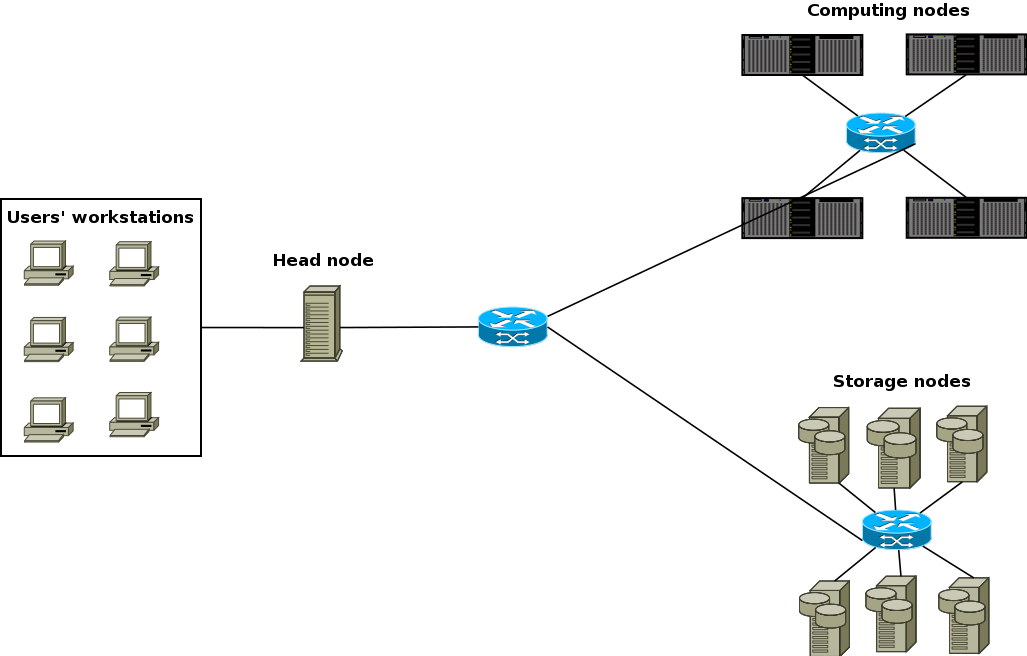
\includegraphics[scale=0.35]{resources/images/Background/hpc_arch_overview.png}
\label{fig:back_hpc_arch_overview}
\caption{HPC high level architecture}
\end{figure}

In 2003 Google published a paper describing GoogleFS (GFS)
\cite{Ghemawat:2003:GFS:1165389.945450}, a proprietary distributed
file system. It was designed to run on large clusters of commodity
hardware, that are doomed to fail at some time. That was the main
motivation that drove GFS to be fault-tolerant and
highly-available. Apache HDFS is the open-source implementation of GFS
and it will be analyzed in Section \ref{ssec:hdfs}. In 2004 Google
published MapReduce \cite{Dean:2004:MSD:1251254.1251264}, a breakthrough programming model which exploited the locality
awareness of GFS and changed the way we process very big
datasets. MapReduce was later implemented for Hadoop and paved the way
for YARN, the current resource manager and scheduler 
which will be analyzed in Section \ref{ssec:yarn}.


\chapter{Method}
\label{chap:method}
%% What are your goals? (What should you be able to do as a result of your solution - which couldn't be done well before you started?)
%%  What you are going to do? Why?
This is going to be the method

\chapter{Analysis}
\label{chap:analysis}
%% How you are going to evaluate what you have done?
%% Analysis of your data and proposed solution
%% Does this meet the goals which you had when you started?
This is going to be the analysis...

\chapter{Conclusions}
\label{chap:conclusion}

\section{Conclusion}
\label{sec:conclusion}
In Hops-YARN, as it is already mentioned, MySQL Cluster NDB is used
both as a communication transport and as a persistent storage for
recovery. At the beginning of the project a thorough profiling of the
execution workflow has been done to identify the bottlenecks of the
system. The first step was to remove the foreign key constraints from
the database schema used by Hops-YARN. In Section
\ref{sec:fk_constraints} is explained how they were replaced by
application logic that performs primary key operations. Section
\ref{sec:tx_aggregation} discusses the evolution of the commit
mechanism which squashes several blocked transaction into a ``big''
one reducing the number of commits in the back-end database
system. Section \ref{sec:gc_service} presents the Garbage Collector
service of Hops-YARN that removes asynchronously old values from the
database. With that solution the commit time dropped more improving
the overall performance of the system. Finally, Section
\ref{sec:dto_caching} explains how the shortcoming of ClusterJ for
creating DTOs was bypassed by having created them ahead of time in a
per session cache.

After a detailed explanation of the solutions proposed, in Chapter
\ref{chap:evaluation} follows the evaluation. Each solution is
evaluated separately by simulating real world traces. In each case key
characteristics are examined and how they have been improved. In
Section \ref{sec:performance_overview} there is an overall performance
overview in terms of cluster utilization and heartbeats processed by
the scheduler. The comparison is made among the version of Hops-YARN
before this project, the final version with all the modification
proposed and the upstream Apache YARN. The figures show that there was
a clear improvement, in both evaluation parameters, when the two
version of Hops-YARN are compared. Finally, as far as the cluster
utilization is concerned, the performance is comparable with Apache
YARN in clusters with thousands of nodes.

\subsection{Goals}
\label{ssec:goals}
In Chapter \ref{chap:introduction} the goals of this project were
set. The primary goals was to improve the cluster utilization and the
number of heartbeats processed by the scheduler. In order to achieve
those goals we have also set some sub-goals. With the solutions proposed
in Chapter \ref{chap:implementation} all the sub-goals were met. In
particular, with the removal of the foreign key constraints and the
DTO caching mechanism the transactional commit time was decreased
dramatically. Some sort of asynchronous API was provided by the
garbage collector service. It is provided only for a small sub-set but
still it made big difference to the performance of the system. The new
aggregation mechanism of the transaction manager of Hops-YARN helped
the blocked transactions to be committed faster which in turn improved the
parallelization of the system. Finally, in each step of the
implementation an evaluation was done to prove the performance impact
and guide us to new bottlenecks.

Since all the sub-goals were met it was expected to achieve the
primary goals. As Chapter \ref{chap:evaluation} indicates the two
primary goals were also accomplished. Both cluster utilization and the
heartbeat ratio was improved.


\subsection{Insights and suggestions for further work}
\label{ssec:insights-and-suggestions}
This is the insights section

\section{Future work}
\label{sec:future-work}
A few things have been left undone due to time limitation and are
discussed in this section for future work.

In most of the cases the evaluation has been done using simulations
measuring among others the cluster utilization while in others the
evaluation has been done using benchmarks. It would be more complete
if in all cases the benchmarks were supported by simulation
results. That way the performance improvements introduced by each step
would be more clear.

Currently we do not have any insight on the content of Transaction
State objects, thus they are treated equally. In real world scenarios,
during the allocation of resources, the Transaction State would carry
more information about allocated containers than when the cluster is
full and no further allocations can be made. A fine-grained inspection
on the content of a TS might improve performance further more. For
example in the commit mechanism, when an Aggregated Transaction State
object is overloading NDB, the transaction will roll-back and the
aggregation policy will enforce a lower limit. If we had any
information on the content of the TS before hand, this situation could
have been avoided.

As it is already mentioned, the Garbage Collector service does not
perform primary key operations. It was a design decision that would
not complicate the mechanism and burden the commit time by committing
more information. It is worth trying to persist all the columns needed
for the primary keys to be reconstructed and measure the
performance. For sure the deletion time would be lower but it
remains to be proven if that will have any impact on the performance
of Hops-YARN in general.

Last but not least, the batching system explained in Section
\ref{ssec:impl_batch_system} should be improved. Changing the number
of RPCs that are batched together did not change the
performance. Every RPC arriving in the ResourceManager among others it
should get the current Transaction State object from the Transaction State
Manager. This operation could take $0.06$ ms. If we consider a cluster
with 10000 NodeManagers heartbeating every second, it is needed 600 ms
just to acquire the object. At the time of writing that was the latest
bottleneck encountered and for sure it is worth for future investigation.

\subsection{What has been left undone?}
\label{ssec:what-has-been-left-undone}
This is what has been left undone


\bibliography{report}
%%\bibliographystyle{IEEEtran}
%%\bibliographystyle{unsrturl}
%%\bibliographystyle{unsrtnat}
\bibliographystyle{myIEEEtran}
\appendix
\chapter{Insensible Approximation}

\backmatter

\end{document}
